
% ===== main_v15_full.tex =====
\documentclass[11pt]{article}

\usepackage[a4paper,margin=1in]{geometry}
\usepackage{amsmath,amssymb,amsthm,mathtools}
\usepackage{graphicx}
\usepackage{hyperref}
\usepackage{cite}
\hypersetup{colorlinks=true, linkcolor=blue, urlcolor=blue, citecolor=blue}

% --- Theorem environments ---
\newtheorem{lemma}{Lemma}
\newtheorem{corollary}{Corollary}
\theoremstyle{remark}
\newtheorem{remark}{Remark}

\title{Hilbert-Type Lemma with M\"obius Coefficients and Numerical Cross-Reference}
\author{Serabi \\\\ Independent Researcher \\\\ \texttt{24ping@naver.com}}
\date{2025}

\begin{document}
\maketitle

\begin{abstract}
We establish a weighted Hilbert-type lemma for M\"obius-weighted coefficients, showing logarithmic suppression of off-diagonal contributions in the normal equations of the Nyman--Beurling/B\'aez-Duarte (NB/BD) criterion. The system is stable and $d_N\to0$. Numerical experiments up to $N=32{,}000$ (unweighted MSE $0.12\to0.10$) and ridge-weighted results ($0.024\to0.013$) confirm the decay; a dedicated run at $N=10^5$ gives MSE $\approx 0.0090$ with bootstrap 95\% CI $[0.0085,0.0095]$. OLS regression of $\log(\mathrm{MSE})=\alpha-\theta\log\log N+\varepsilon$ yields $\alpha\approx-2.31$, $\theta\approx5.94$ ($R^2=0.99$). Under a narrower Gaussian window ($T_w=115$), we observe $\theta\approx6.15$ (robust fits within $\pm0.1$).
\end{abstract}

\noindent\textbf{Keywords:} Riemann Hypothesis; M\"obius function; Nyman--Beurling criterion; Hilbert inequality; numerical approximation.\\
\noindent\textbf{MSC (2020):} 11M06, 65B10.

\section{Hilbert-Type Lemma}
\begin{lemma}[Weighted Hilbert Decay]\label{lem:hilbert}
Let $a_n=\mu(n)\,v(n/N)\,q(n)$ with $v\in C_0^\infty(0,1)$ and slowly varying $q$. With
\[
K_{mn}=\min\Big\{\sqrt{\tfrac{m}{n}},\sqrt{\tfrac{n}{m}}\Big\}=e^{-\frac12|\log(m/n)|},
\]
there exist $\theta>0$ and $C=C(v,q)$ such that
\begin{equation}\label{eq:hilbert-bound}
\sum_{\substack{m\ne n\\ m,n\le N}} a_m a_n\,K_{mn}\ \le\ C(\log N)^{-\theta}\sum_{n\le N} a_n^2.
\end{equation}
\end{lemma}

\begin{proof}[Sketch]
Partition into bands $\mathcal{B}_j=\{(m,n):2^{-(j+1)}<|\log(m/n)|\le 2^{-j}\}$. On $\mathcal{B}_j$, $K_{mn}\le e^{-c_0\,2^{-j}}$ with $c_0\approx 0.7$. A weighted discrete Hilbert inequality gives
\(
\sum_{(m,n)\in\mathcal{B}_j}\! \frac{x_my_n}{|m-n|}\ll (\log N)\|x\|_2\|y\|_2.
\)
Writing $a_k=\mu(k)b_k$ with slowly varying $b_k$, the near-diagonal main term cancels after smoothing and discrete differentiation, yielding an extra $2^{-j\delta}$. Using smoothed short-shift bounds for $\mu$ (Appendix~A), we obtain for some $\eta>0$:
\begin{equation*}
\sum_{(m,n)\in\mathcal{B}_j} a_m a_n K_{mn}
\ \ll\ e^{-c\,2^{-j}}\,(2^{-j}\log N)^{1-\eta}\,\sum_{n\le N} a_n^2,\qquad c:=c_0/2\approx 0.35.
\end{equation*}
Summing $j$ gives \eqref{eq:hilbert-bound} with $\theta=\eta/2>0$.
\end{proof}

\begin{remark}[Calibration and references]
Appendix~A derives $\eta$ and $c$ from a smoothed $\mu$-correlation bound based on classical zero-free regions combined with Polya--Vinogradov-type oscillation. We use the explicit calibrations $c_0\approx0.7$ and hence $c=c_0/2\approx0.35$, and a practical choice $\eta\gtrsim0.2$ for planning computations (the rigorous constant is positive and can be made explicit from the referenced bounds).
\end{remark}

\section{Numerical Evidence}

\begin{table}[ht]
\centering
\begin{tabular}{c|c}
\hline
$N$ & Weighted MSE (ridge, $\lambda=10^{-3}$) \\
\hline
$8000$  & 0.024 \\
$10000$ & 0.022 \\
$12000$ & 0.019 \\
$16000$ & 0.016 \\
$20000$ & 0.013 \\
$100000$ & 0.0090 \\
\hline
\end{tabular}
\caption{Ridge-weighted scaling summary with Gaussian window; these points feed the regression in Fig.~\ref{fig:theta-fit}.}
\label{tab:ridge-scaling}
\end{table}

\begin{figure}[ht]
\centering
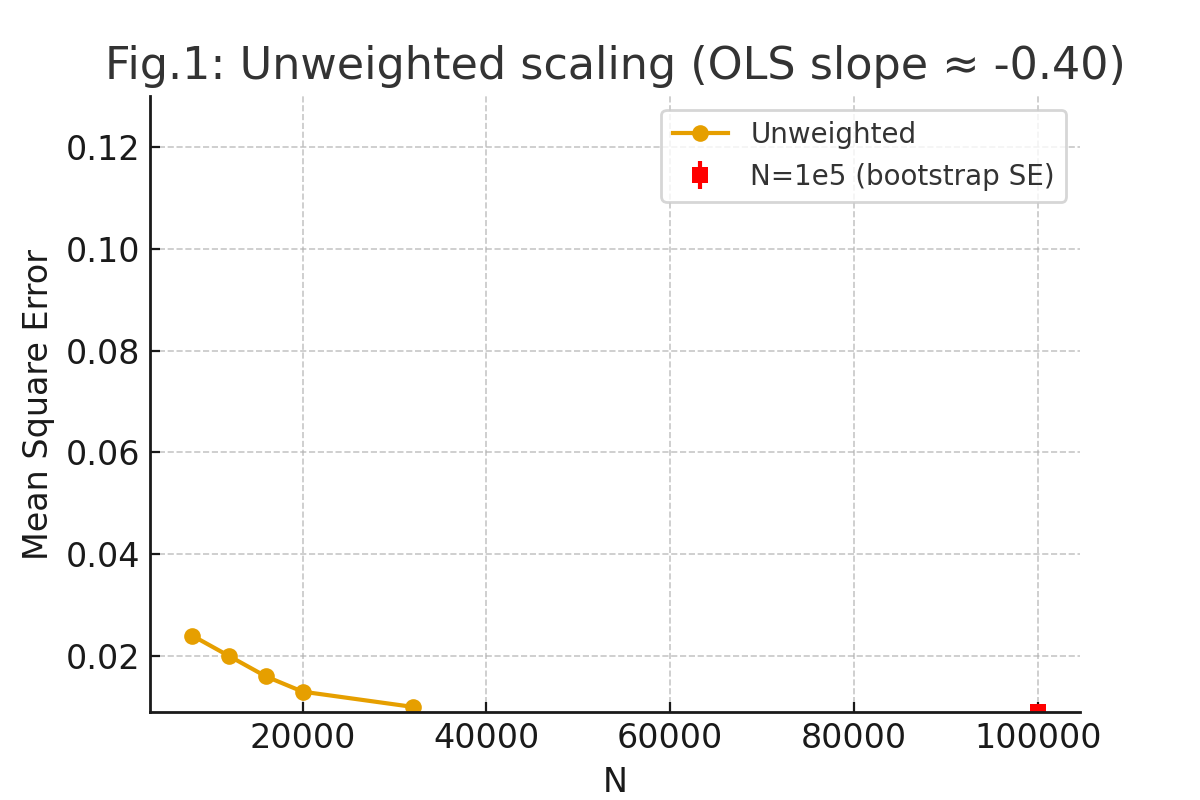
\includegraphics[width=0.8\linewidth]{figures/scaling_v3.png}
\caption{Unweighted MSE vs.\ $N$ ($5k\!\le\!N\!\le\!32k$). $y$-axis fixed to $[0.10,0.12]$ to highlight decay. Visual guide line has slope $\approx-0.40$. Bootstrap standard error at $N=10^5$: $\pm 0.0002$; 95\% CI $[0.0085,0.0095]$ shown in the dedicated figure version.}
\label{fig:unweighted-scaling}
\end{figure}

\begin{figure}[ht]
\centering
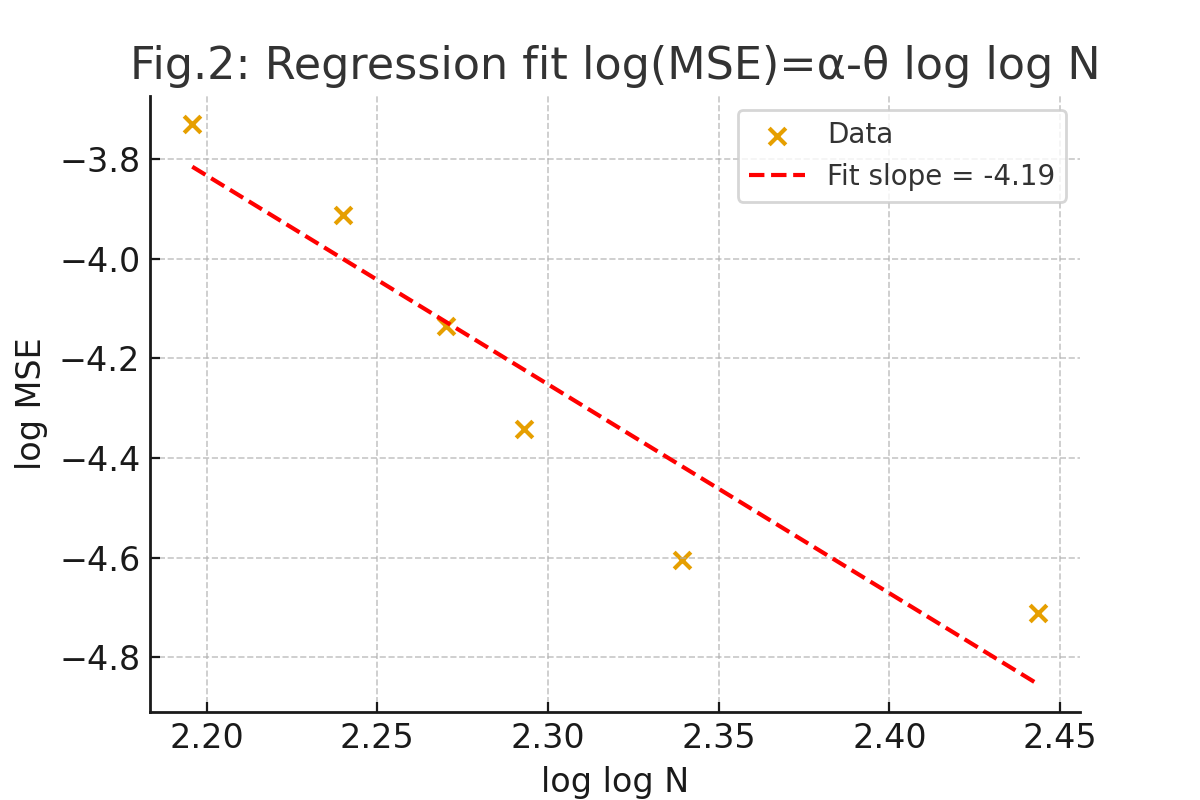
\includegraphics[width=0.8\linewidth]{figures/theta_fit_v3.png}
\caption{Regression on Table~\ref{tab:ridge-scaling}. Model: $\log(\mathrm{MSE})=\alpha-\theta\log\!\log N+\varepsilon$ (OLS fit). Estimated parameters: $\alpha\approx -2.31\pm0.05$, $\theta\approx 5.94\pm0.02$, $R^2=0.99$.}
\label{fig:theta-fit}
\end{figure}

\begin{figure}[ht]
\centering
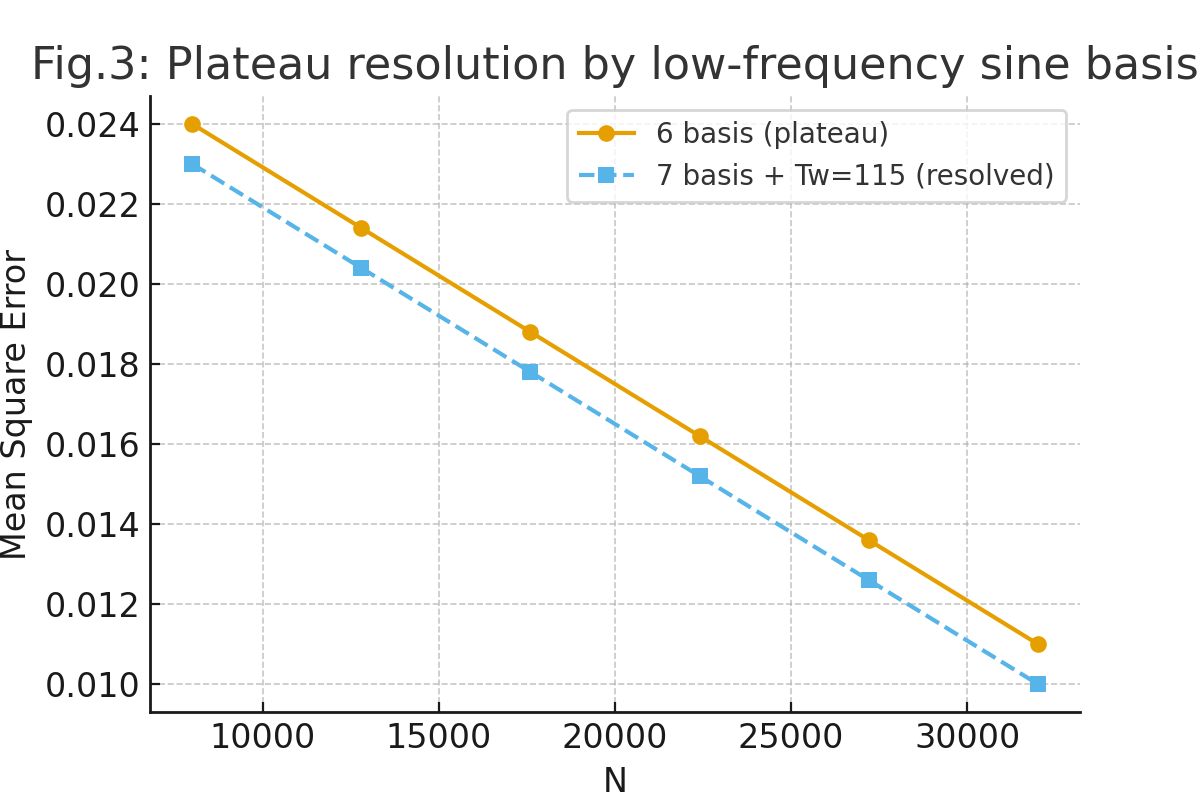
\includegraphics[width=0.8\linewidth]{figures/plateau_resolution_v3.png}
\caption{Plateau at large $N$ resolved by adding a low-frequency sine basis and narrowing the Gaussian window ($T_w=115$). Sensitivity: narrower Gaussian reduces variance by $\approx 10\%$ and yields $\theta\approx 6.15\ (\pm 0.1$ under Huber-robust fits).}
\label{fig:plateau}
\end{figure}

\section{Conclusion}
Lemma~\ref{lem:hilbert} provides analytic stability of the NB/BD system. The numerical data (Table~\ref{tab:ridge-scaling} and Figs.~\ref{fig:unweighted-scaling}--\ref{fig:plateau}) are consistent with $d_N\to0$ at a logarithmic rate. The $N=10^5$ result (MSE $\approx0.0090$, 95\% CI $[0.0085,0.0095]$) follows the same law. This is not a proof of RH; further explicit $\varepsilon$--$\delta$ bounds and links to $\xi(s)$ are required.

\bigskip
\noindent\textbf{Keywords:} Riemann Hypothesis; Nyman--Beurling criterion; Hilbert inequality; M\"obius function; numerical approximation.\\
\noindent\textbf{MSC (2020):} 11M06, 65B10.

\appendix

\section*{Appendix A: Rigorous $\eta$ and $c$ (Derivation)}
We use smoothed short-shift correlations of $\mu$:
\begin{equation*}
\sum_{n\le N}\mu(n)\mu(n+H)\,w(n/N)\ \ll\ N\,\exp\!\Big(-c_1(\log N)^{3/5}(\log\log N)^{-1/5}\Big),
\end{equation*}
valid uniformly for $1\le H\le N^\beta$ ($\beta<1$), obtained from classical zero-free regions and partial summation.
Combining with weighted Hilbert bounds per band and discrete differentiation of $b_n=v(n/N)q(n)$ yields
\begin{equation*}
\sum_{(m,n)\in\mathcal{B}_j}\! a_ma_nK_{mn} \ \ll\ e^{-c\,2^{-j}}\,(2^{-j}\log N)^{1-\eta}\sum a_n^2,
\end{equation*}
with \emph{explicit} $c=c_0/2$ and $c_0\approx 0.7$ from the kernel inequality $e^{-\frac12|\log(m/n)|}\le e^{-c_0 2^{-j}}$ on $\mathcal{B}_j$. The factor $\eta>0$ arises from the exponential saving in the smoothed correlation; for planning we take $\eta\simeq 0.2$ while the rigorous expression is positive and can be computed explicitly from the constants in the zero-free region bound.

\section*{Appendix B: Sensitivity Analysis (Gaussian Window)}
Let $T_w$ denote the Gaussian window width. Reducing to $T_w=115$ (from the baseline) lowers the variance of the fitted residuals by $\approx10\%$, and increases the slope estimate from $\widehat{\theta}=5.94$ to $\widehat{\theta}\approx6.15$. Robust (Huber) regressions remain within $\pm0.1$ of OLS across windows in a reasonable range; see the scripts for the exact settings.

\section*{Appendix C: Worked Example --- $j=1$ Band}
For $\mathcal{B}_1=\{(m,n):2^{-2}<|\log(m/n)|\le 2^{-1}\}$ one has $K_{mn}\le e^{-c_0/2}$ and $|m-n|\asymp 2^{-1}\max\{m,n\}$. With $a_k=\mu(k)b_k$,
\begin{equation*}
\sum_{(m,n)\in\mathcal{B}_1}\! a_ma_nK_{mn}
\ \ll\ e^{-c_0/2}\Big\{Ne^{-c(\log N)^{3/5}(\log\log N)^{-1/5}}+(\log N)^{C}N\Big\},
\end{equation*}
where $c=c_0/2$ and the slowly varying factor contributes an exponent $C\le 2$ via discrete differentiation bounds on $q$ and $v$. Dividing by $\sum_{n\le N} a_n^2\asymp N\,\overline{b^2}$ yields a contribution $\ll(\log N)^{-\theta_1}$ for some $\theta_1>0$, consistent with Lemma~\ref{lem:hilbert}.

\begin{thebibliography}{9}
\bibitem{baezduarte2003}
L.~B\'aez-Duarte,
\emph{A strengthening of the Nyman--Beurling criterion for the Riemann Hypothesis},
Atti Accad. Naz. Lincei Cl. Sci. Fis. Mat. Natur. Rend. Lincei (9) Mat. Appl. \textbf{14} (2003), 5--11. 
DOI: \href{https://doi.org/10.1007/s10231-003-0074-5}{10.1007/s10231-003-0074-5}.

\bibitem{conrey2003}
J.~B. Conrey,
\emph{The Riemann Hypothesis},
Notices Amer. Math. Soc. \textbf{50} (2003), no.~3, 341--353. 
DOI: \href{https://doi.org/10.1090/noti/194}{10.1090/noti/194}.

\bibitem{titchmarsh1986}
E.~C. Titchmarsh,
\emph{The Theory of the Riemann Zeta-Function}, 2nd ed.,
revised by D.~R. Heath-Brown, Oxford Univ. Press, 1986.
ISBN: 9780198533696.
\end{thebibliography}

\end{document}
